\documentclass{beamer}
\mode<presentation> {
\usepackage{color}
\definecolor{bottomcolour}{rgb}{0.21,0.11,0.21}
\definecolor{middlecolour}{rgb}{0.21,0.11,0.21}
\setbeamercolor{structure}{fg=white}
\setbeamertemplate{frametitle}[default]%[center]
\setbeamercolor{normal text}{bg=black, fg=white}
\setbeamertemplate{background canvas}[vertical shading]
[bottom=bottomcolour, middle=middlecolour, top=black]
\setbeamertemplate{items}[circle]
\setbeamertemplate{navigation symbols}{} %no nav symbols
\setbeamercolor{block title}{use=structure,fg=white,bg=structure.fg!50!red!50!blue!100!green}
\setbeamercolor{block body}{parent=normal text,use=block title,bg=block title.bg!5!white!10!bg,fg=white}
\setbeamertemplate{navigation symbols}{}
}
\usepackage{graphicx} 
\usepackage{booktabs} 
\usepackage[utf8]{inputenc}  
\usepackage{geometry}     
%\usepackage[francais]{babel} 
\usepackage{eurosym}
\usepackage{verbatim}
\usepackage{ragged2e}
\justifying

%%%%%%%%%%%%%%%%%%%%%%%%%%%%%%%%%%%%%%%%%%%%%%%%%%%%%%%%%%%%%%%%
%% ccBeamer 0.1, 2007-07-02                                   %%
%% Written by Sebastian Pipping <webmaster@hartwork.org>      %%
%% ---------------------------------------------------------- %%
%% Licensed under Creative Commons Attribution-ShareAlike 3.0 %%
%% http://creativecommons.org/licenses/by-sa/3.0/             %%
%%%%%%%%%%%%%%%%%%%%%%%%%%%%%%%%%%%%%%%%%%%%%%%%%%%%%%%%%%%%%%%%


%% Images
\newcommand{\CcImageBy}[1]{%
	
\includegraphics[scale=#1]{creative_commons/cc_by_30.pdf}%
}
\newcommand{\CcImageCc}[1]{%
	
\includegraphics[scale=#1]{creative_commons/cc_cc_30.pdf}%
}
\newcommand{\CcImageDevNations}[1]{%
	
\includegraphics[scale=#1]{creative_commons/cc_dev_nations_30.pdf}%
}
\newcommand{\CcImageNc}[1]{%
	
\includegraphics[scale=#1]{creative_commons/cc_nc_30.pdf}%
}
\newcommand{\CcImageNd}[1]{%
	
\includegraphics[scale=#1]{creative_commons/cc_nd_30.pdf}%
}
\newcommand{\CcImagePd}[1]{%
	
\includegraphics[scale=#1]{creative_commons/cc_pd_30.pdf}%
}
\newcommand{\CcImageSa}[1]{%
	
\includegraphics[scale=#1]{creative_commons/cc_sa_30.pdf}%
}
\newcommand{\CcImageSampling}[1]{%
	
\includegraphics[scale=#1]{creative_commons/cc_sampling_30.pdf}%
}
\newcommand{\CcImageSamplingPlus}[1]{%
	
\includegraphics[scale=#1]{creative_commons/cc_sampling_plus_30.pdf}%
}


%% Groups
\newcommand{\CcGroupBy}[1]{% zoom
	\CcImageBy{#1}%
}
\newcommand{\CcGroupByNc}[2]{% zoom, gap
	\CcImageBy{#1}\hspace*{#2}\CcImageNc{#1}%
}
\newcommand{\CcGroupByNcNd}[2]{% zoom, gap
	\CcImageBy{#1}\hspace*{#2}\CcImageNc{#1}\hspace*{#2}\CcImageNd{#1}%
}
\newcommand{\CcGroupByNcSa}[2]{% zoom, gap
	\CcImageBy{#1}\hspace*{#2}\CcImageNc{#1}\hspace*{#2}\CcImageSa{#1}%
}
\newcommand{\CcGroupByNd}[2]{% zoom, gap
	\CcImageBy{#1}\hspace*{#2}\CcImageNd{#1}%
}
\newcommand{\CcGroupBySa}[2]{% zoom, gap
	\CcImageBy{#1}\hspace*{#2}\CcImageSa{#1}%
}
\newcommand{\CcGroupDevNations}[1]{% zoom
	\CcImageDevNations{#1}%
}
\newcommand{\CcGroupNcSampling}[2]{% zoom, gap
	\CcImageNc{#1}\hspace*{#2}\CcImageSampling{#1}%
}
\newcommand{\CcGroupPd}[1]{% zoom
	\CcImagePd{#1}%
}
\newcommand{\CcGroupSampling}[1]{% zoom
	\CcImageSampling{#1}%
}
\newcommand{\CcGroupSamplingPlus}[1]{% zoom
	\CcImageSamplingPlus{#1}%
}


%% Text
\newcommand{\CcLongnameBy}{Attribution}
\newcommand{\CcLongnameByNc}{Attribution-NonCommercial}
\newcommand{\CcLongnameByNcNd}{Attribution-NoDerivs}
\newcommand{\CcLongnameByNcSa}{Attribution-NonCommercial-ShareAlike}
\newcommand{\CcLongnameByNd}{Attribution-NoDerivs}
\newcommand{\CcLongnameBySa}{Attribution-ShareAlike}

\newcommand{\CcNote}[1]{% longname
	This work is licensed under the \textit{Creative Commons #1 3.0 License}.%
}

\title[L'identité numérique]{L'identité numérique} 
\author{Genma}
\begin{document}
%% Titlepage
\begin{frame}
	\titlepage
	\vfill
	\begin{center}
		\CcGroupByNcSa{0.83}{0.95ex}\\[2.5ex]
		{\tiny\CcNote{\CcLongnameByNcSa}}
		\vspace*{-2.5ex}
	\end{center}
\end{frame}

%----------------------------------------------------------------------------------------
\begin{frame}
\begin{center}
\Huge{Introduction}
\end{center}
\end{frame}

%----------------------------------------------------------------------------------------
\begin{frame}
\begin{center}
\justifying{
Identité réelle/virtuelle, e-réputation, droit à l’oubli  : notre identité sur le net peut-elle être maîtrisée de la même façon que dans le monde physique ? 
}
\end{center}
\begin{center}
\justifying{
Comment contrôler son image ? Peut-on dire que nous avons aujourd’hui deux vies, l’une sur internet (sur les réseaux sociaux, les sites de rencontre par exemple) et l’autre près de nos proches et des gens que nous côtoyons?}
\end{center}
\end{frame}

%----------------------------------------------------------------------------------------
\begin{frame}
\begin{center}
\justifying{
C'est à cet ensemble de questions à ces problématiques que je vais tenter de répondre, en me basant sur ma propre expérience...
}
\end{center}
\end{frame}

%----------------------------------------------------------------------------------------
\begin{frame}
\frametitle{Qui suis-je?}

\begin{block}{Jérôme...}
\begin{itemize}
\justifying{
\item C'est mon prénom civil.
\item Cette identité numérique existe, mais dans le cadre de la gestion de mon e-reputation.
}
\end{itemize}
\justifying{Ne pas être présent en ligne est \emph{presque} suspect...}
\end{block}

\begin{block}{mais surtout Genma!}
\begin{itemize}
\justifying{
\item Auteur du blog \emph{le Blog de Genma} \url{http://genma.free.fr} depuis 2004
\item Identité numérique publique, assez forte (Réseaux sociaux) et \emph{cohérente}.
}
\end{itemize}
\end{block}
\end{frame}
%----------------------------------------------------------------------------------------
\begin{frame}
\begin{center}
\Huge{L'identité numérique}
\end{center}
\end{frame}

%----------------------------------------------------------------------------------------
\begin{frame}
\frametitle{L'identité numérique c'est quoi?}

\begin{block}{Définition}
\begin{itemize}
\justifying{
\item L'identité numérique, c'est l'ensemble des données publiques que l'on peut trouver sur Internet et rattacher à une personne.
}
\end{itemize}
\end{block}
\end{frame}

%----------------------------------------------------------------------------------------
\begin{frame}
\frametitle{L'identité numérique c'est quoi?}

\begin{block}{Définition}
\begin{itemize}
\justifying{
\item L'identité numérique, c'est l'ensemble des données publiques que l'on peut trouver sur Internet et rattacher à une personne, en l'occurrence moi.
}
\end{itemize}
\end{block}
\end{frame}

%-----------------------------------------------
\begin{frame}
\frametitle{E-réputation}

\begin{block}{Par où commencer ?}
\begin{itemize}
\justifying{
\item Quelle image je donne de moi ?
\item Que trouve-t-on sur moi comme informations quand on tape mes "nom, prénom" dans un moteur de recherche ?
}
\end{itemize}
\end{block}

\begin{block}{Les questions à de poser}
\begin{itemize}
\justifying{
\item Suis en capacité d'assumer tout ce que l'on trouve sur moi ? De le justifier ?
\item Est-ce qu'il y a des choses que je voudrais cacher ?
\item Que je regrette ?
}
\end{itemize}
\end{block}
\end{frame}
%-----------------------------------------------
\begin{frame}
\frametitle{Taper son nom dans Google}
\begin{center}
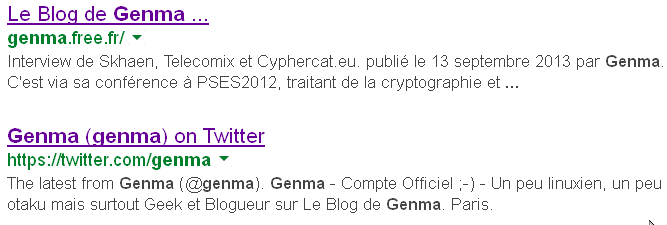
\includegraphics[scale=0.5] {./images/Google01.png} 
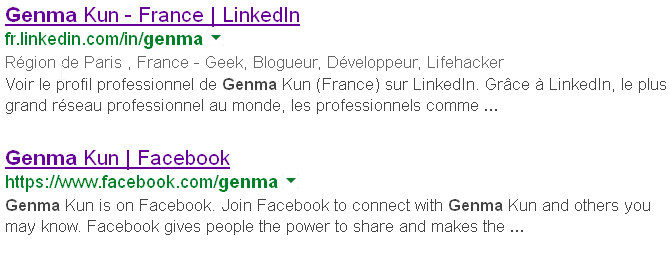
\includegraphics[scale=0.5] {./images/Google02.png} 
\end{center}
\end{frame}
%-----------------------------------------------
\begin{frame}
\huge{
La quasi totalité des informations que l'on trouve sur nous, ce sont des informations que NOUS avons mises en ligne (via les réseaux sociaux par exemple).}
\end{frame}

%----------------------------------------------------------------------------------------
\begin{frame}
\frametitle{Adage}
\begin{block}{Les paroles s'envolent, les écrits restent}
\begin{itemize}
\justifying{
\item Cet adage est encore plus vrai avec Internet.
\item  Il faut partir du principe que ce que l'on dit sera toujours accessible, même des années après.
\item Tout ce qui est sur Internet est public ou le sera (même si c'est "privé". Les conditions d'utilisation évoluent. Cf. Facebook).
\item Il ne faut donc pas abuser de la liberté d'expression et rester respectueux des lois en vigueur.
}
\end{itemize}
\end{block}
\end{frame}


%----------------------------------------------------------------------------------------
\begin{frame}
\frametitle{La netiquette}

\begin{block}{Définition}
\justifying{
La nétiquette est une règle informelle, puis une charte qui définit les règles de conduite et de politesse recommandées sur les premiers médias de communication mis à disposition par Internet. Il s'agit de tentatives de formalisation d'un certain contrat social pour l'Internet.
}
\end{block}
\justifying{
En résumé ce sont les règles de savoir-vivre et de respect que l'on devrait tou-te-s avoir sur Internet.}
\end{frame}

%----------------------------------------------------------------------------------------
\begin{frame}
\begin{center}
\Huge{Le droit à l’oubli}
\end{center}
\end{frame}

%-----------------------------------------------
\begin{frame}
\frametitle{Le droit à l’oubli}

\begin{block}{Définition}
\justifying{
Il permet à un individu de demander le retrait de certaines informations qui pourraient lui nuire sur des actions qu'il a faites dans le passé. 
\\~\\
Le droit à l'oubli s'applique concrètement soit par le retrait de l'information sur le site d'origine, on parle alors du droit à l'effacement, soit par un déréférencement du site par les moteurs de recherche, on parle alors du droit au déréférencement.
}
\end{block}
\end{frame}

%-----------------------------------------------
\begin{frame}
\frametitle{Les problématiques soulevées par le droit à l'oubli}

\begin{block}{Les questions que cela soulève…}
\begin{itemize}
\justifying{
\item Le droit à l'oubli entre en conflit avec ceux de l'information et de l'expression.
\item Quid de la censure ?
\item Internet n'a pas de frontières…
\item "L'effet Streisand".
}
\end{itemize}
\end{block}
\end{frame}

%----------------------------------------------------------------------------------------
\begin{frame}
\begin{center}
\Huge{Le pseudonymat}
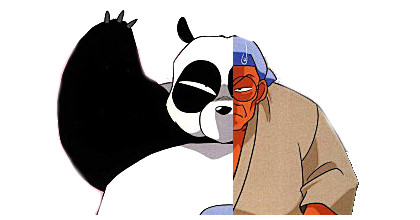
\includegraphics[scale=0.5] {./images/bannierepseudonymat.jpg} 
\end{center}
\end{frame}

%----------------------------------------------------------------------------------------
\begin{frame}
\frametitle{Le pseudonymat}

\begin{block}{Défintions}
\begin{itemize}
\justifying{
\item Contraction des termes pseudonyme et anonymat, le terme de pseudonymat reflète assez bien la volonté contradictoire d’être un personnage public et de rester anonyme...
\item Un pseudonyme, c'est aussi une identité publique, qui est associée à un ensemble cohérent de comptes qui forment un tout : un blog, un compte Twitter, un compte Facebook…
}
\end{itemize}
\justifying{
L'identité numérique est l'ensemble des données publiques associées à cette identité. 
}
\end{block}
\end{frame}

\begin{frame}
\frametitle{Exemples}
\begin{center}
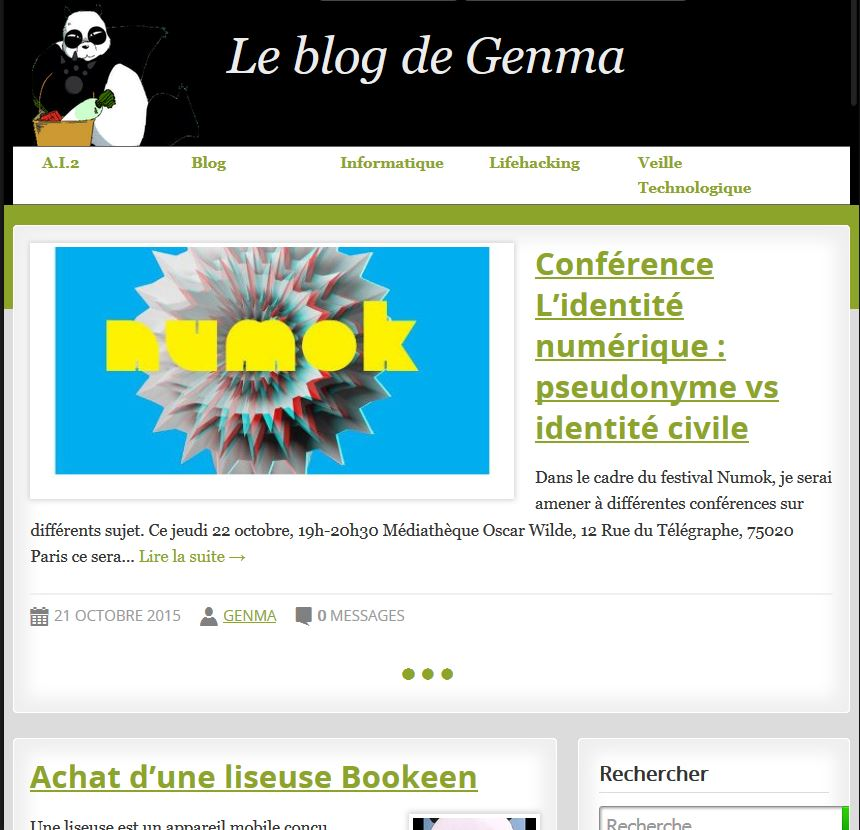
\includegraphics[scale=0.5] {./images/blog.png} 
\end{center}
\end{frame}

\begin{frame}
\frametitle{Exemples}
\begin{center}
Linkedin\\~\\
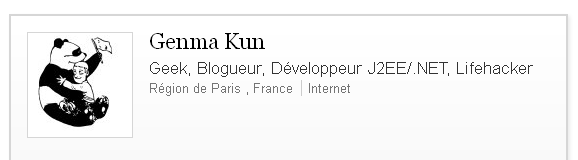
\includegraphics[scale=0.4] {./images/Linkedin.png} 
\\
Twitter @genma\\
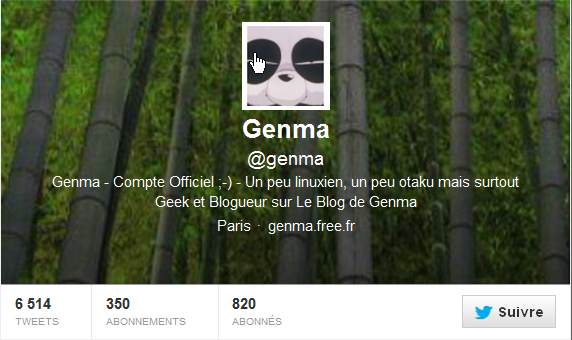
\includegraphics[scale=0.4] {./images/Twitter.png}
\end{center}
\end{frame}

%----------------------------------------------------------------------------------------
\begin{frame}
\frametitle{Le pseudonymat}

\begin{block}{Attention}
\justifying{
Avoir un pseudonyme ne veut pas dire faire et dire n'importe quoi.
\\~\\Il en va de l'image que je renvoie, que je donne de moi et de ma crédibilité présente et à venir.
}
\end{block}
\end{frame}


%----------------------------------------------------------------------------------------
\begin{frame}
\frametitle{Les avantages du pseudonymat}

\begin{block}{Ce que permet le pseudonymat}
\justifying{Il permet de cloisonner sa vie numérique.}
\begin{itemize}
\justifying{
\item On a une une identité civile en ligne (nom, prénom) avec le strict minimum.
\item Et une identité publique, un pseudonyme, qui permet d'avoir une activité plus fournie.
}
\end{itemize}
\end{block}
\justifying{
Ne pas oublier d'avoir une adresse mail qui ne soit pas de la forme prénom.nom (sinon on perd l'intérêt du pseudonyme).
}
\end{frame}

%----------------------------------------------------------------------------------------
\begin{frame}
\frametitle{Plusieurs pseudonymes}

\justifying{
Quand on crée un compte sur un site, on peut envisager de saisir des informations nominatives spécifiques à ce site. On aura alors un pseudonyme par type de communauté fréquenté (jeu vidéo, informatique, de rencontres...).
\\~\\
S’il y a un problème (\emph{compte piraté}), on limitera le risque de diffusion des informations personnelles.
}
\end{frame}

%----------------------------------------------------------------------------------------
\begin{frame}
\frametitle{Pseudonymat et célébrité}

\justifying{Nombreuses sont les célébrités du monde de la télévision, cinéma, musique… Et Internet?}
\begin{block}{Des pseudonymes internet \emph{connus}}
\begin{itemize}
\justifying{
\item Maitre Eolas, l'avocat
\item Zythom, l'expert judiciaire
\item Boulet, dessinateur
\item ...
}
\end{itemize}
\end{block}
\justifying{Et beaucoup d'autres, dans les communautés geek, hackers...}
\end{frame}

%----------------------------------------------------------------------------------------
\begin{frame}
\frametitle{Les limites du pseudonymat}

\begin{block}{Un pseudonymat c'est contraignant}

\justifying{On est très facilement tracés et reliés à sa véritable identité (via l'adresse IP).}
\begin{itemize}
\justifying{
\item Pour avoir un pseudonymat parfaitement cloisonné, il faut utiliser différentes techniques avancées…
}
\end{itemize}
\end{block}

\begin{block}{NE JAMAIS faire d'erreur}
\begin{itemize}
\justifying{
\item On ne dévoile pas son pseudonyme a des personnes qui connaissent notre identité civile.
\item On ne dévoile pas son visage en public…
}
\end{itemize}
\end{block}
\justifying{
Le pseudonymat est donc on ne peut plus relatif et tout dépend de ce que l'on souhaite comme pseudonymat.
}
\end{frame}

%----------------------------------------------------------------------------------------
\begin{frame}
\frametitle{L'anonymat}

\justifying{
Il est possible d'être anonyme sur Internet. Mais cela est TRÈS compliqué et la moindre erreur (qui ne sera pas toujours celle à laquelle on pense, voir le cas de Silk Road) fera que l'on n'est plus anonyme.
\\~\\
Il est \emph{assez facile} de retrouver l'auteur d'un commentaire diffamatoire, raciste ou autre (tant que ce dernier n'a pas utilisé d'outil d'anonymisation avancé comme Tor).
}
\end{frame}

%----------------------------------------------------------------------------------------
\begin{frame}
\begin{center}
\Huge{Les \emph{risques} des réseaux sociaux}
\end{center}
\end{frame}


%----------------------------------------------------------------------------------------
\begin{frame}
\frametitle{Les risques des réseaux sociaux}

\begin{block}{Centralisation des données}
\justifying{
En un seul endroit (Facebook par exemple), il y a énormément d'informations personnelles qui sont cumulées.
\begin{itemize}
\item Ces données peuvent être accessibles par n'importe qui, si le compte est \emph{mal configuré}.
\item Risque d'attaque de type \emph{social engineering}.
\end{itemize}
}
\end{block}

\begin{block}{Si c'est gratuit, c'est vous le produit}
\justifying{
\begin{itemize}
\item Ces données sont revendues et exploitées.
\end{itemize}
}
\end{block}

\justifying{
D'où l'importance de se créer une identité numérique sous pseudonyme, sur laquelle on a un contrôle \emph{relatif}.
}

\end{frame}

%----------------------------------------------------------------------------------------
\begin{frame}
\begin{center}
\Huge{Conclusion}
\end{center}
\end{frame}

%-----------------------------------------------
\begin{frame}
\frametitle{Conclusion}

\begin{block}{
\justifying{La maîtrise de son identité numérique en ligne repose avant tout sur soi-même}}
\begin{itemize}
\justifying{
\item Il ne faut pas \emph{tout} dire ou mettre sur les réseaux sociaux ;
\item Il faut essayer de compartimenter ses différentes vies numériques (en sachant jusqu'où on veut et jusqu'où on est prêt à aller).
}
\end{itemize}
\end{block}

\begin{block}{
\justifying{Sur Internet, on ne fait pas n'importe quoi}}
\begin{itemize}
\justifying{
\item On est responsable des propos que l'on tient vis-à-vis de la loi.
\item L'anonymat existe mais est \emph{presque} une utopie.
}
\end{itemize}
\end{block}
\end{frame}

%----------------------------------------------------------------------------------------
\begin{frame}
\begin{center}
\Huge{Merci de votre attention. \\~\\ Place aux questions.}
\end{center}
\end{frame}

%----------------------------------------------------------------------------------------
\begin{frame}
\begin{center}
\Huge{Annexes}
\end{center}
\end{frame}


%----------------------------------------------------------------------------------------
\begin{frame}
\frametitle{Qui a modifié quoi sur Wikipedia ?}
\begin{center}
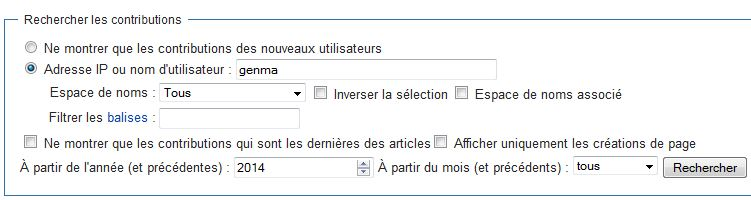
\includegraphics[scale=0.7] {./images/wikpedia_ip.jpg} 
\end{center}
\end{frame}

\begin{frame}
\frametitle{Comment un pseudonymat peut voler en éclat ?}
\begin{itemize}
\justifying{
\item En publiant sur les réseaux sociaux
\item Message du répondeur de son téléphone portable
\item On se trompe de boite mail...
}
\end{itemize}
\end{frame}

\begin{frame}
\begin{center}
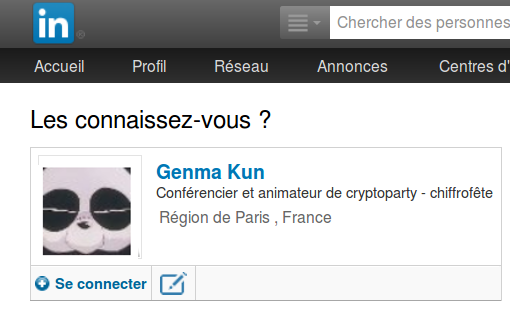
\includegraphics[scale=0.7] {./images/attention_cookies_linkedin.png} 
\end{center}
\end{frame}




\end{document}